\documentclass[11pt]{article}
\usepackage[a4paper, portrait, margin=1in]{geometry}
\usepackage{mathtools}
\usepackage{listings}
\usepackage[dvipsnames]{xcolor}
\usepackage{color}
\usepackage{graphicx}
\usepackage[colorlinks=true,urlcolor=blue,linkcolor=black]{hyperref}


\DeclarePairedDelimiter{\ceil}{\lceil}{\rceil}

\newcommand{\code}[1]{\lstinline[language=Java]{#1}}
\newcommand{\get}[0]{\texttt{GET}}
\newcommand{\set}[0]{\texttt{SET}}
\newcommand{\todo}[1]{\fcolorbox{black}{Apricot}{TODO: #1}}
\newcommand{\linkmain}[1]{\href{https://gitlab.inf.ethz.ch/pungast/asl-fall16-project/blob/master/src/main/java/asl/#1.java}{#1}}
\newcommand{\linktest}[1]{\href{https://gitlab.inf.ethz.ch/pungast/asl-fall16-project/blob/master/src/test/java/asl/#1.java}{#1}}

\newcommand{\resultsurl}[1]{\href{https://gitlab.inf.ethz.ch/pungast/asl-fall16-project/blob/master/results/#1}{gitlab.inf.ethz.ch/.../results/#1}}




\begin{document}

\title{Advanced Systems Lab (Fall'16) -- Second
Milestone}

\author{Name: \emph{Taivo Pungas}\\Legi number: \emph{15-928-336}}

\date{
\vspace{4cm}
\textbf{Grading} \\
\begin{tabular}{|c|c|}
\hline  \textbf{Section} & \textbf{Points} \\ 
\hline  1 &  \\ 
\hline  2 &  \\ 
\hline  3 &  \\ 
\hline \hline Total & \\
\hline 
\end{tabular} 
}

\maketitle

\newpage

\tableofcontents

\clearpage
% --------------------------------------------------------------------------------
% --------------------------------------------------------------------------------
\section*{Modifications to the middleware}
% --------------------------------------------------------------------------------
% --------------------------------------------------------------------------------
\addcontentsline{toc}{section}{Modifications to the middleware}

In the last milestone submission, my middleware implemented all functionality as necessary. However, the resource usage was extremely wasteful: each read thread took up nearly 100\% of the resources allocated to them and never went to a sleeping state. This caused more than 10-fold drops in performance when going from $T=1$ to $T=4$ (for $S=5$), and would have made the maximum throughput experiment useless. The changes can be seen on \href{https://gitlab.inf.ethz.ch/pungast/asl-fall16-project/commit/928e9bba132d34ecf9c00936babdd7fa2645e50f}{GitLab}.

To verify that the system is still stable, I re-ran the trace experiment. The throughput and response time are shown in Figures~\ref{fig:trace:throughput} and \ref{fig:trace:responsetime}, and are confirmed to be stable (and throughput is roughly 30\% higher). The Interactive Response Time Law also still holds (to within 0.46\%). For explanations of the figures, see Milestone 1 report.

\begin{figure}[h]
\centering
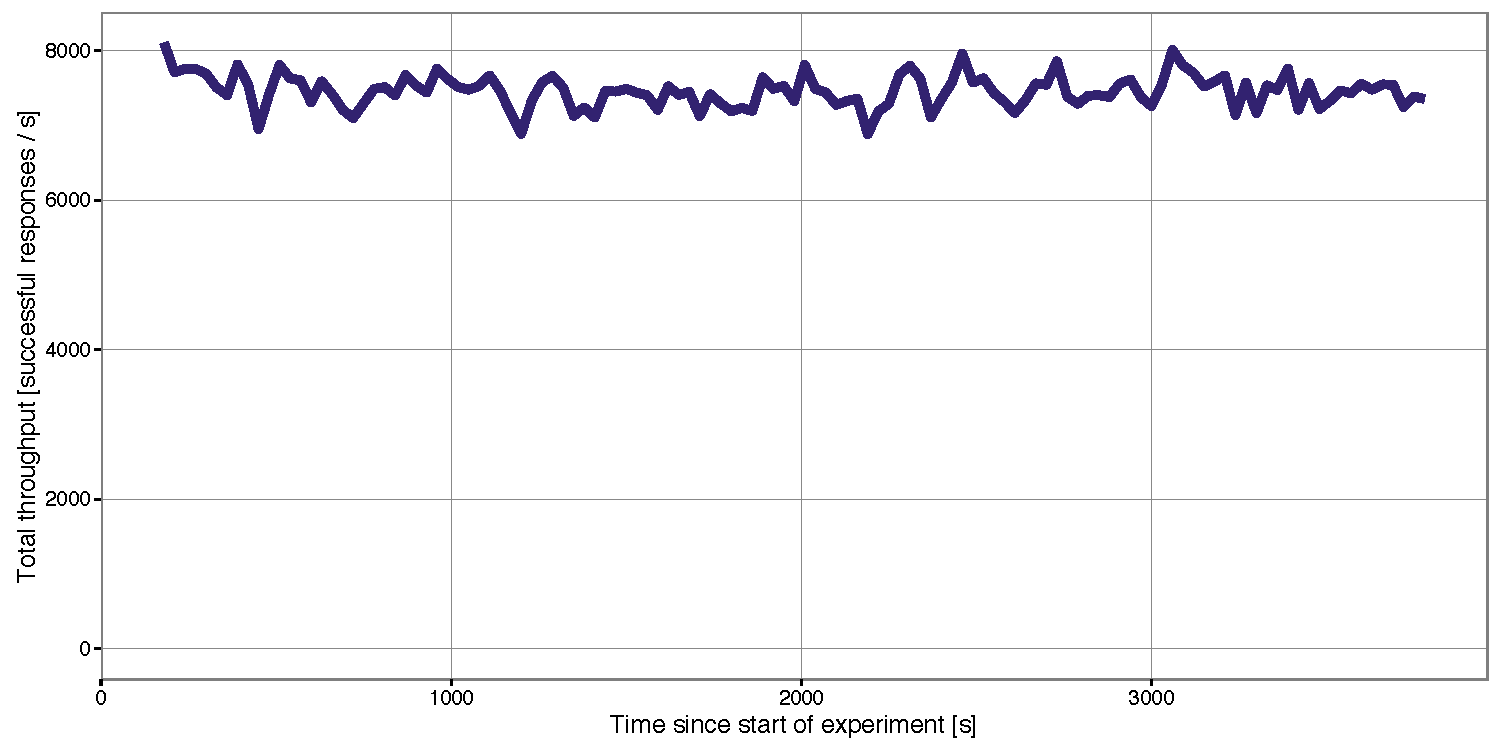
\includegraphics[width=\textwidth]{../results/trace_rep3/graphs/throughput.pdf}
\caption{Throughput trace of the middleware.}
\label{fig:trace:throughput}
\end{figure}

\begin{figure}[h]
\centering
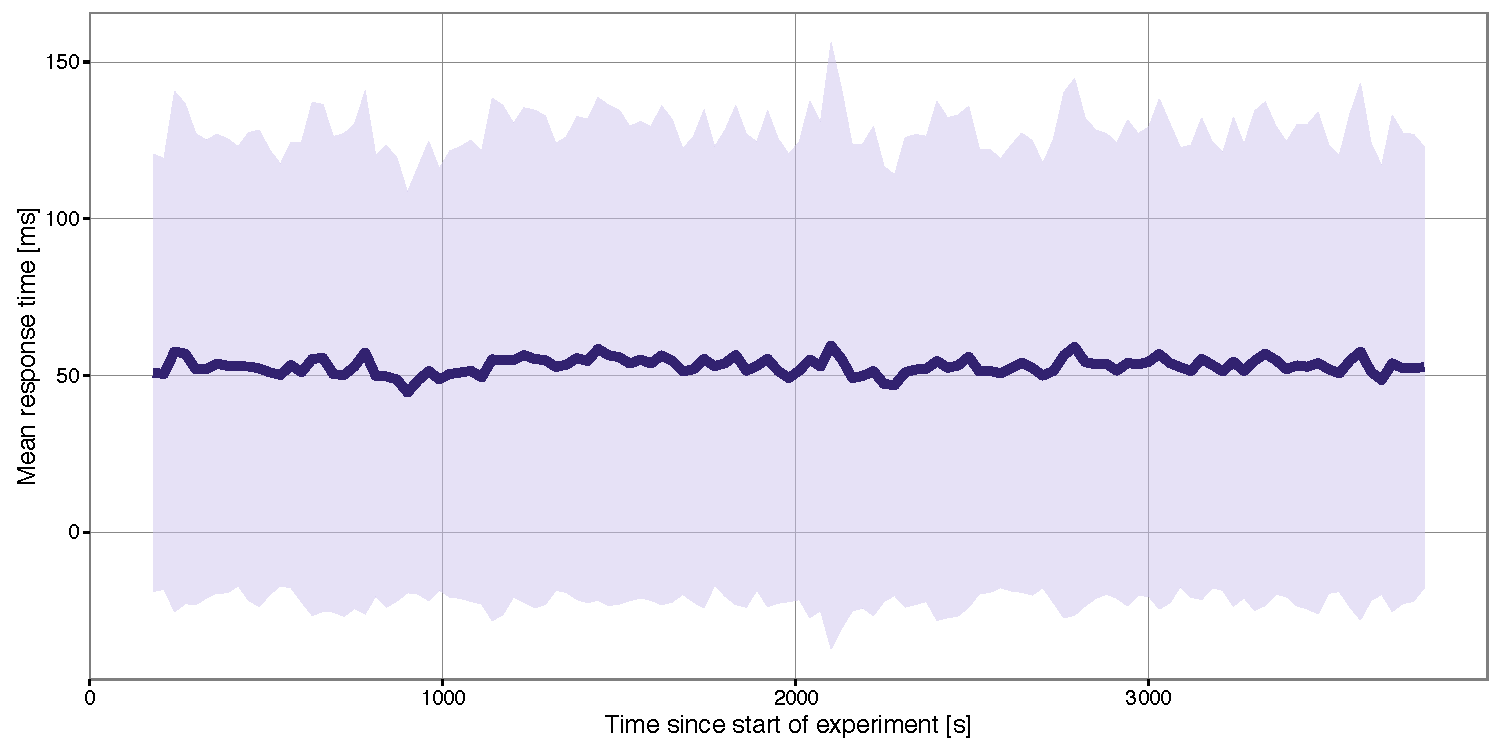
\includegraphics[width=\textwidth]{../results/trace_rep3/graphs/responsetime.pdf}
\caption{Response time trace of the middleware as measured by memaslap.}
\label{fig:trace:responsetime}
\end{figure}


% --------------------------------------------------------------------------------
% --------------------------------------------------------------------------------
\section*{Definitions and setup}
% --------------------------------------------------------------------------------
% --------------------------------------------------------------------------------
\addcontentsline{toc}{section}{Definitions and setup}

In all experiments, the following definitions hold.

\begin{itemize}
\item The \emph{system under test} (SUT) is the middleware together with the connected memcached servers, running on Ubuntu virtual machines in the Azure cloud.
\item \emph{Throughput} is the number of requests the SUT successfully responds to, per unit of time, as measured by memaslap.
\item \emph{Response time (memaslap)} is the time from sending to receiving the request to the SUT including any network latencies, as measured by the client (memaslap).
\item \emph{Response time (middleware)} is the time from receiving the request in the middleware ($t_{created}$) to returning it to the client ($t_{returned}$), as measured by the middleware. This is the measurement used in most graphs here; the reasoning behind this is shown in \hyperref[sec:appa]{Appendix A}.
\end{itemize}

In all experiments, the following holds about the experimental setup:
\begin{itemize}
\item The middleware was run on Basic A4 instances, and both memaslap and memcached were run on Basic A2 instances.
\item The first 2 and last 2 minutes of each experiment were discarded from analyses as warm-up and cool-down time.
\item The request sampling rate for logging is set to $\frac{1}{100}$ in throughput experiments (Section~\ref{sec:exp1}) and $\frac{1}{10}$ in replication and write proportion experiments (Sections~\ref{sec:exp2} and \ref{sec:exp3}).
\item Response times inside the middleware were measured with a 1 millisecond accuracy.
\item The system is closed because memaslap clients wait for a response before sending a new request.
\end{itemize}


\clearpage
% --------------------------------------------------------------------------------
% --------------------------------------------------------------------------------
\section{Maximum Throughput}
% --------------------------------------------------------------------------------
% --------------------------------------------------------------------------------
\label{sec:exp1}

\subsection{Experimental question}

In this section, I will run experiments to find out a) the maximum throughput of the SUT, b) the number of read threads ($T$) in the middleware that achieves this c) the number of virtual clients ($C$) that achieves this.

To this end, I will measure throughput as a function of $T$ and $C$, in 10-second time windows. I will find the maximum sustained throughput of the SUT, i.e. the throughput at which the response time does not increase rapidly with additional clients. For each parameter combination, I will run experiments until the 95\% confidence interval (calculated using a two-sided t-test) lies within 5\% of the mean throughput.

\subsection{Hypothesis}

I approximate that the maximum throughput will be 17200 requests per second using 50 read threads in the middleware at a load of 550 clients. The maximum sustained throughput will occur in a range of 200 clients.

\subsubsection{Number of threads} 
Given that requests spend most of their time ($\sim90\%$ in the trace experiment) waiting in the queue, increasing $T$ will increase throughput. If we reduce the queueing time by a factor of 10, it will no longer be the bottleneck (then waiting for memcached's response -- which takes $\sim9\%$ of response time in the trace experiment -- becomes the bottleneck). Assuming the time spent in the queue scales linearly with the number of read threads, we should increase $T$ 10-fold, i.e. $T=50$ maximises throughput.

\subsubsection{Number of clients}
Throughput is maximised at roughly 110 virtual clients per memcached server, so 550 virtual clients in total. This is based on the fact that in the Milestone 1 baseline experiment, the throughput of a single memcached server without middleware saturated at around 110 virtual clients. However, the knee of the graph was at 40 to 50 clients per server, so we can expect the knee to occur at around 200 clients in our setup. The maximum sustained throughput will be in that region because after the knee, additional clients don't increase throughput much but significantly increase response time.

\subsubsection{Throughput}
In the trace experiment the throughput was roughly 10300 requests per second so we have a lower bound for the expected throughput. Naively assuming that the throughput of \get{} requests scales linearly with the number of servers $S$ would yield an expected throughput of $\frac{5}{3} \cdot 10300 = 17200$ requests per second. However, this does not take into account that we will also increase the number of threads (from $T=5$ in the trace experiment). Thus I expect the maximum sustained throughput to be definitely more than 10300 requests per second, and likely to be more than 17200 requests per second.

I predict that the graph of throughput as a function of the number of clients will look like in Figure~\ref{fig:exp1:hyp:throughput}: rapidly increasing at first, then reaching the knee after which throughput growth is much slower, and then completely saturating. After saturation, the throughput may fall due to unexpected behaviour in the middleware.

\paragraph{Breakdown of response time}
I expect that the most expensive operations inside the middleware will be queueing ($t_{dequeued}-t_{enqueued}$) and waiting for a response from memcached ($t_{forwarded}-t_{received}$). Queueing takes time because for a $C$ that gives a high throughput, the queue will also be non-empty and requests will need to wait. Requesting a response from memcached takes time because of a) the time it takes for memcached to process the request and b) the round-trip network latency.

\begin{figure}[h]
\centering
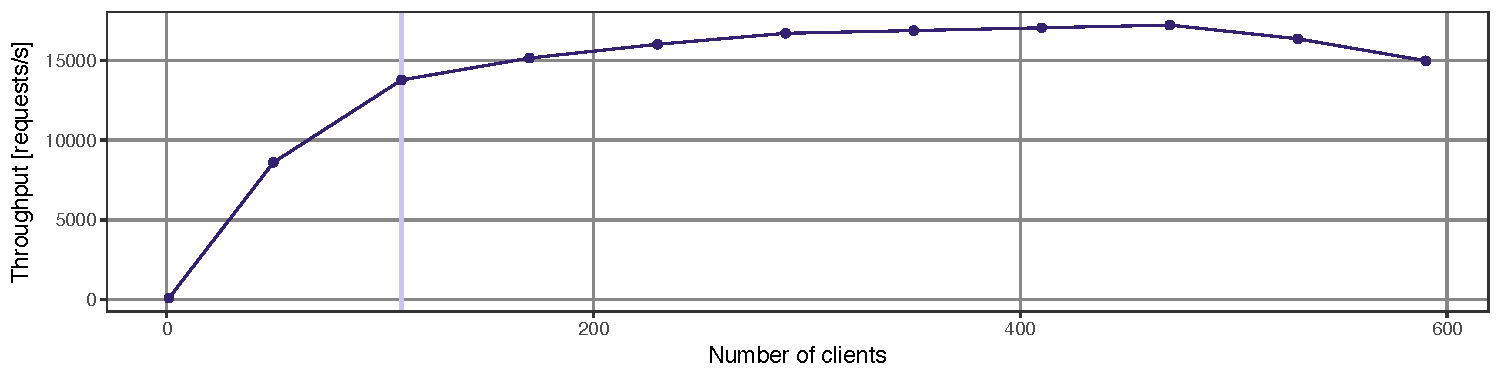
\includegraphics[width=\textwidth]{figures/hypothesis_throughput.pdf}
\caption{Expected graph of throughput as a function of number of clients (for the optimal value of $T$). The shaded area shows the range where maximum sustained throughput (and knee of the graph) will occur.}
\label{fig:exp1:hyp:throughput}
\end{figure}

\subsection{Experiments}
\begin{center}
\small{
\smallskip
\begin{tabular}{|c|c|}
\hline Number of servers & 5 \\ 
\hline Number of client machines & $\in \{1, 3\}$ \\ 
\hline Virtual clients & $\in \{1, 36, 72, 144, 180, 216, 288, 360, 432, 504, 576, 648\}$ \\ 
\hline Workload & Key 16B, Value 128B, Writes 0\% \\
\hline Middleware: replication factor & 1 \\ 
\hline Middleware: read threads & $\in\{1, 16, 32, 64\}$ \\ 
\hline Runtime x repetitions & at least 6min x 1; more in some cases \\ 
\hline Log files & throughput-C*-T*-r* \\
\hline 
\end{tabular} }
\end{center}

Three client machines were used for all experiments, except for the 1-client experiment, where only one machine was used.

The values of $T$ to test were $T=1$ as the lowest possible value, and then from $T=16$ in multiplicative steps of 2. The reason for the small number of tested values of $T$ is pragmatic: it doesn't require hundreds of experiments and at the same time gives a reasonable approximation of the optimal $T$.

Some parameter combinations did not yield the required confidence interval in the first 6-minute repetition of the experiment. When that was the case, I re-ran the experiment (in some cases for a longer time), thus producing more datapoints and decreasing the confidence interval.

\subsection{Results}
\todo{restructure with subsubsections}

\paragraph{Maximum sustained throughput}
Figure~\ref{fig:exp1:res:throughput} shows that the highest throughput was achieved using $T=64$ at 720 clients (20100 requests/s), followed by $T=64$ at 648 clients (20000 requests/s) and $T=32$ at 432 clients (19600 requests/s). This is reasonably close to the expected value of $C=550$. However, since we are trying to maximise sustained throughput, we also need to look at response times.

Figure~\ref{fig:exp1:res:responsetime} shows the percentiles of the response time distribution for each parameter set. It is apparent that for all values of $T > 1$, both the median response time (green line) and 95\% quantile (blue line) increase significantly after 216 clients. For this reason, we will exclude all values of $T > 216$ from consideration as unsustainable.

Of the remaining setups, the highest throughput is achieved both by 180 and 216 clients at $T=32$. Thus we pick the one with the lower number of clients -- \textbf{180 clients and 32 threads} -- as the configuration we will declare optimal at a throughput of 18400 requests per second. Both $C$ and throughput are close to the expected values; $T$ is lower but not by an order of magnitude.

\todo{Explain} why the system reaches its maximum throughput at these points and show how the performance changes around these configurations.

\paragraph{Breakdown of response time} The distribution of time \get{} requests spend in different parts of the middleware is shown in Figure~\ref{fig:exp1:res:breakdown}, and the means in Figure~\ref{fig:exp1:table}. As expected, the most expensive operations are queueing and waiting for a response from memcached. The distributions of $tQueue$ and $tMemcached$ are bimodal with a second peak at roughly 8ms because \todo{why?}.

\begin{figure}[h]
\centering
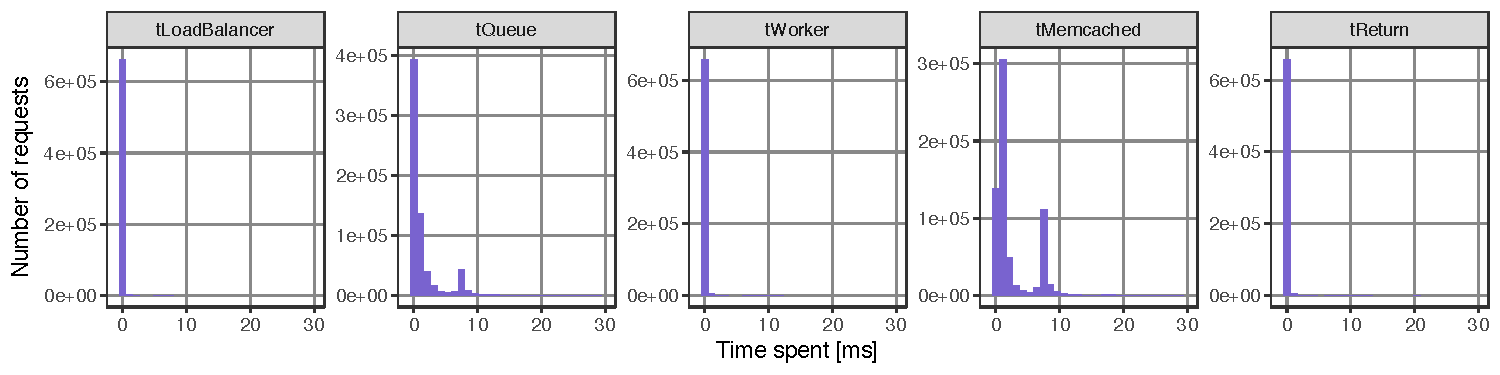
\includegraphics[width=\textwidth]{../results/throughput/graphs/response_time_breakdown.pdf}
\caption{The distribution of times that \get{} requests spend in different parts of SUT. Note the time axis only shows values up to 30ms (this range includes almost all datapoints).}
\label{fig:exp1:res:breakdown}
\end{figure}

\begin{figure}[h]
\begin{center}
	\begin{tabular}{|c|c|c|l |}
	\hline \textbf{Name} & \textbf{Begin timestamp} & \textbf{End timestamp} & \textbf{Mean [ms]} \\
	\hline tLoadBalancer & $t_{created}$ & $t_{enqueued}$ & 0.0043 \\
	\hline tQueue & $t_{enqueued}$ & $t_{dequeued}$ & 1.40 \\
	\hline tWorker & $t_{dequeued}$ & $t_{forwarded}$ & 0.0191 \\
	\hline tMemcached & $t_{forwarded}$ & $t_{received}$ & 2.85 \\
	\hline tReturn & $t_{received}$ & $t_{returned}$ & 0.0221 \\
	\end{tabular}
	\caption{The amount of time spent on different operations inside the middleware for the optimal run ($C=180$ and $T=32$), for \get{} requests.}
	\label{fig:exp1:table}
\end{center}
\end{figure}

\begin{figure}[p]
\centering
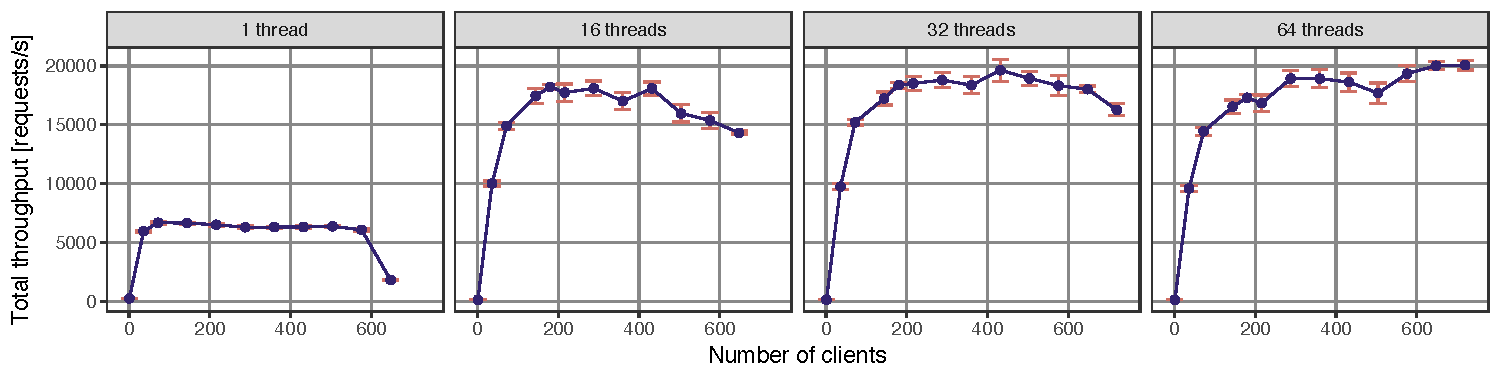
\includegraphics[width=\textwidth]{../results/throughput/graphs/tp_vs_clients.pdf}
\caption{Throughput as a function of $C$ for different values of $T$. Errorbars show the 95\% confidence interval around the mean value which is shown with points connected by lines.}
\label{fig:exp1:res:throughput}
\end{figure}

\begin{figure}[p]
\centering
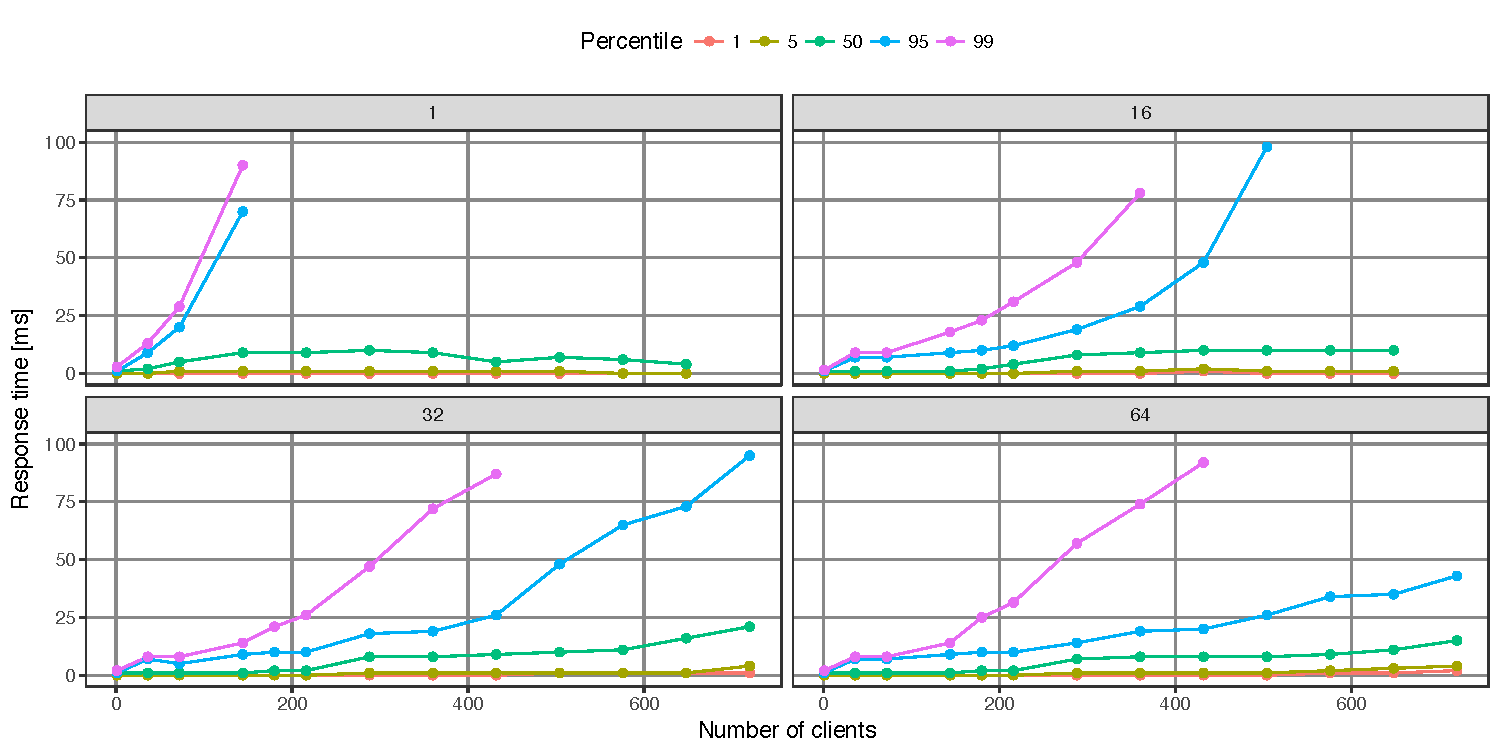
\includegraphics[width=\textwidth]{../results/throughput/graphs/response_time_vs_clients.pdf}
\caption{The 1\%, 5\%, 50\%, 95\% and 99\% percentiles of the response time (middleware) distribution, as a function of $C$ for different values of $T$. Values above 100ms are not shown.}
\label{fig:exp1:res:responsetime}
\end{figure}



\clearpage
% --------------------------------------------------------------------------------
% --------------------------------------------------------------------------------
\section{Effect of Replication}
% --------------------------------------------------------------------------------
% --------------------------------------------------------------------------------
\label{sec:exp2}

\subsection{Experimental question}

In this section, I will run experiments to find out how the response time of SUT depends on the number of servers $S$ and replication factor $R$. Additionally, I will investigate whether \get{}s and \set{}s are differently affected by these parameters. Finally, I will find out which operations become more time-consuming as these parameters change.

To this end, I will measure response time (middleware) for every 10th request as a function of $S$ and $R$, and measure how long requests spend in each part of the SUT (based on the timestamps defined in Milestone 1). For each parameter combination, I will run experiments until the 95\% confidence interval (calculated using a two-sided t-test) lies within 5\% of the mean response time, but not less than 3 repetitions.

\subsection{Hypothesis}

I predict the following.

\subsubsection{\get{} and \set{} requests}
\get{} and \set{} requests will not be impacted the same way by different setups.

\get{} requests will be processed faster as we increase $S$ because the same load will be distributed across more threads. Increasing $R$ will have no effect on \get{} requests because replication is only done for \set{} requests (there may be secondary effects due to e.g. write threads requiring more CPU time, but this should be negligible).

\set{} requests will be strongly affected by $R$. If $R=1$, \set{} requests will be processed faster for higher $S$ because each request is only written to one server, and for a higher $S$ the same load is distirbuted across more write threads. However, if $R>1$, response time of \set{}s increases due to two factors: a) the request is written serially to $R$ servers, and b) not all $R$ responses are received at the same time. Assuming a) is negligible compared to b), we will observe an increase in the mean response time.

All of this is summarised in Figure~\ref{fig:exp2:hyp:replication}. For \get{} requests, response time will be independent of $R$ for any fixed $S$. For \set{} requests, response time increases linearly with increasing $R$, and the slope increases with $S$.

\begin{figure}[h]
\centering
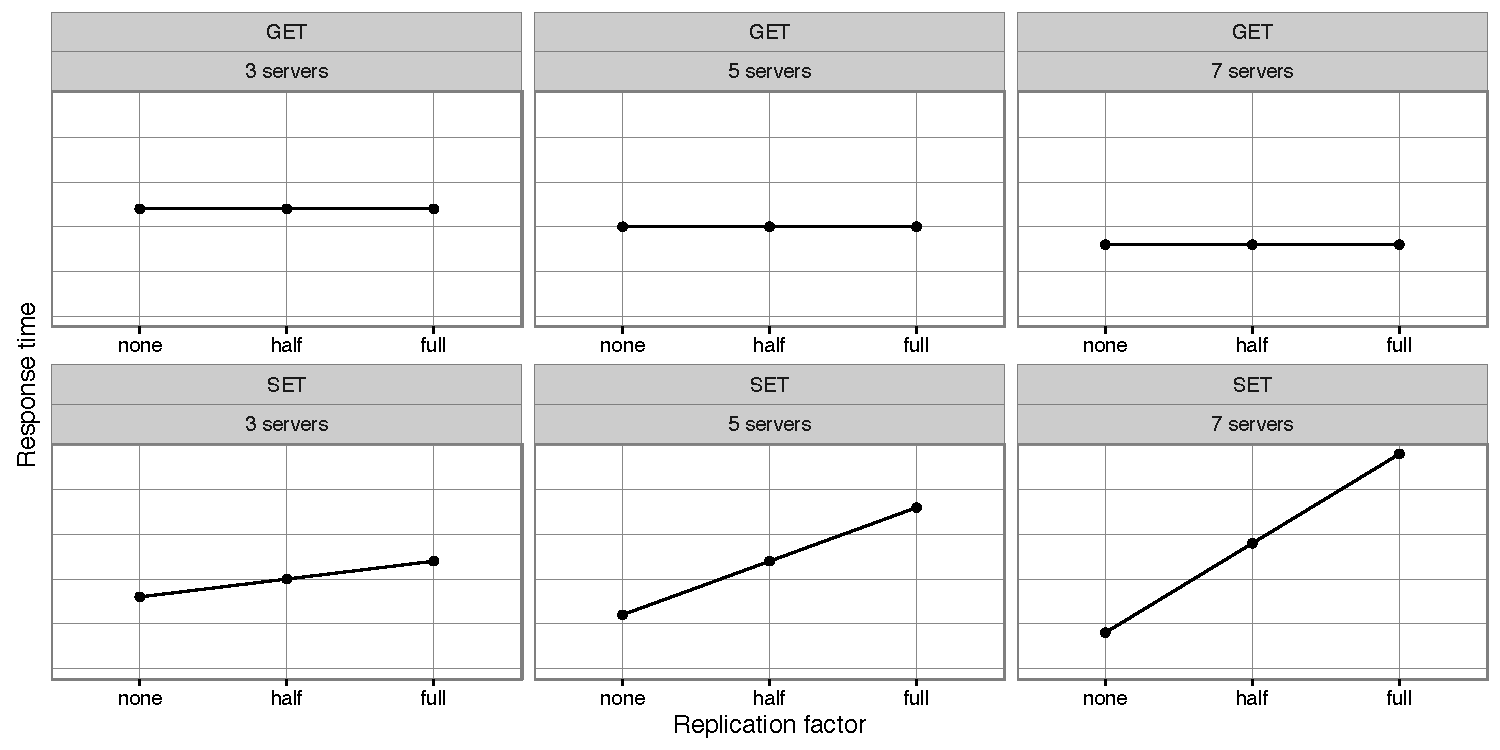
\includegraphics[width=\textwidth]{figures/hypothesis_replication.pdf}
\caption{Expected response times of SUT. The vertical (time) axis has an arbitrary but fixed scale for all plots in the top row, and a different but also fixed scale for the bottom row.}
\label{fig:exp2:hyp:replication}
\end{figure}


\subsubsection{Throughput}
I also predict the total throughput will decrease as $R$ increases because the servers will need to do additional work (communicating more with memcached servers).

\subsubsection{Relative cost of operations}
As explained previously, more replication means that the middleware needs to send each \set{} request to more servers and wait for more answers. Thus, as $R$ increases, $tMemcached$ will increase. Since each \set{} request takes longer to process, this means that $tQueue$ will increase as well. I also predict that the relative cost of \get{} operations will not change.

\subsubsection{Scalability}
\label{sec:exp2:hyp:scalability}

In an ideal system, a) there would be enough resources to concurrently run all threads; b) all memcached servers would take an equal and constant amount of time to respond; c) there would be no network latencies; d) dequeueing would take constant time.

For \get{} requests, the ideal system would have linear speed-up (assuming the load balancer does not become a bottleneck). I predict that the SUT will have sublinear speed-up because the response time also includes network latency -- a term that is not dependent on $S$: $response \; time = const. + \frac{const.}{S}$. In addition, since threads compete for resources in the SUT, the speed-up will be even lower than what's predicted by the formula above.

\todo{and for sets?} what's the hypothesis?

\subsection{Experiments}
\begin{center}
\small{
\smallskip
\begin{tabular}{|c|c|}
\hline Number of servers & $\in \{3, 5, 7\}$ \\ 
\hline Number of client machines & 3 \\ 
\hline Virtual clients & 180 \\ 
\hline Workload & Key 16B, Value 128B, Writes 5\% \\
\hline Middleware: replication factor & $\in \{1, ceil(S/2), S\}$ \\ 
\hline Middleware: read threads & 32 \\ 
\hline Runtime x repetitions & 6min x 3 \\ 
\hline Log files & replication-S*-R*-r* \\
\hline 
\end{tabular} }
\end{center}

\subsection{Results}

\subsubsection{\get{} requests}
From Figure~\ref{fig:exp2:res:replication} we can see that increasing $R$ from 1 to $S$ does have an impact on the mean response time of \get{} requests (contrary to the hypothesis) and this effect is amplified as $S$ grows. However, the 25\%, 50\%, and 75\% percentiles stay constant, implying that most of the requests aren't affected (in accordance with the hypothesis) -- only the response time of outliers (\get{}s with high response times) increases. Figure~\ref{fig:exp2:res:breakdown} shows that queue time is constant and the increase in response time comes almost entirely from waiting for memcached's response; this means the increase is caused by either increased network latency (due to more traffic at a higher value of $R$) or increased memcached response time.

I predicted that increasing $S$ while keeping $R$ constant would decrease the response time of \get{} requests. In fact I was only partly right: the 25\%, 50\%, and 75\% percentiles stay constant, but the mean decreases with $S$ at $R=1$ and increases at $R>1$. Investigating the breakdown of time spent inside the middleware (Figure~\ref{fig:exp2:res:breakdown}) gives an answer: queueing time does decrease with $S$ for all replication levels, but this gain is offset by the increase in time spent waiting for memcached's response.

Given that $tMemcached$ increased with $S$ even when $R$ was constant, we can conclude that the performance degradation was mostly due to networking -- if it had been caused by memcached's slower responses, $tMemcached$ would not have changed with $S$.

\subsubsection{\set{} requests}
\label{sec:exp2:res:set}

Figure~\ref{fig:exp2:res:replication} shows that increasing $R$ does increase response time for $S=7$ but unexpectedly, decreases response time for $S=3$. This is counterintuitive: how can a system that is under a higher load also be faster?

From Figure~\ref{fig:exp2:res:breakdown} we see that queueing time actually decreases with $R$ at all values of $S$ and the increase in $tMemcached$ offsets the decrease at $S=5$ and $S=7$. Why, then, do \set{} requests spend less time in the queue as $R$ increases? We can explain this by looking at the architecture of \linkmain{WriteWorker}. Two steps are done in the same loop: first, if the write queue has any elements, one is taken and sent to all $R$ servers. The second step is checking for responses from memcached (waiting up to 1ms using the function \verb+Selector.select(long timeout)+). This means that if there were no responses from memcached servers, the thread just sleeps 1ms.

The result of this design is that a system with a larger replication factor -- which means more responses from memcached servers -- sleeps less at \verb+Selector.select()+ and thus can faster go back to processing elements from the queue.

Adding servers at $R=1$ decreases response time to \set{} requests -- this is in line with the hypothesis. For $R>1$ adding servers does not have a linear effect on response time: for 50\% replication, response time (and the time spent in each component) is constant and at full replication response time increases slightly with $S$ because of increased $tMemcached$.

$tMemcached$ is almost constant at 50\% replication because the difference between values of $R$ is small: $R \in \{2,3,4\}$. At full replication tMemcached has a larger effect because the difference is larger: $R \in \{3,5,7\}$. (The slowest response determines $tMemcached$; it can be modelled as the maximum of $R$ samples where each sample is the response time to one request from the middleware to a memcached server.).

\begin{figure}[h]
\centering
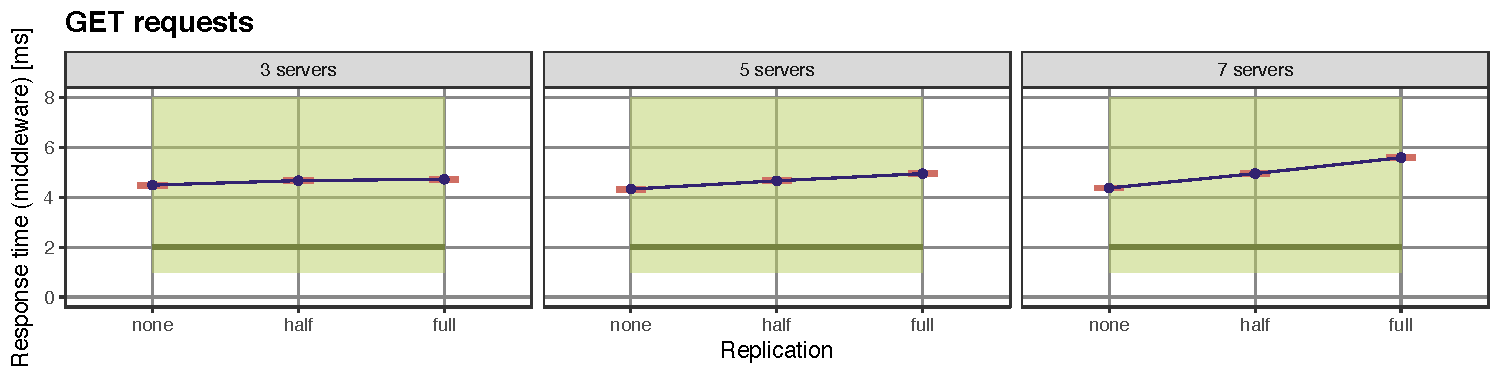
\includegraphics[width=\textwidth]{../results/replication/graphs/response_time_vs_replication_get.pdf}
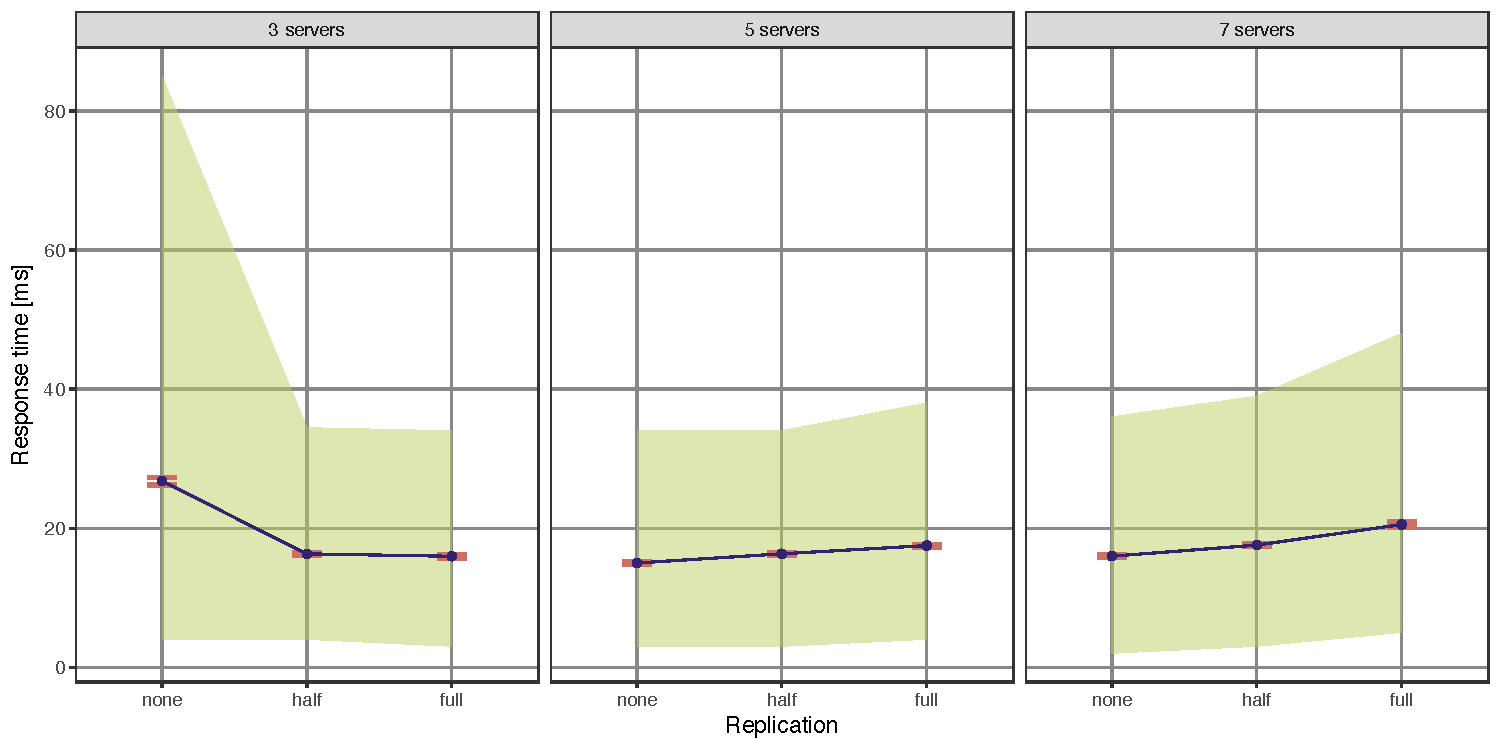
\includegraphics[width=\textwidth]{../results/replication/graphs/response_time_vs_replication_set.pdf}
\caption{Response time (middleware) as a function of $R$, for different values of $S$. The blue line and points show the mean response time; red errorbars show the 95\% confidence interval in a double-tailed t-test; the green area shows the 25\% (bottom edge) and 75\% (top edge) quantiles of response times; the green line shows the median.}
\label{fig:exp2:res:replication}
\end{figure}

\begin{figure}[h]
\centering
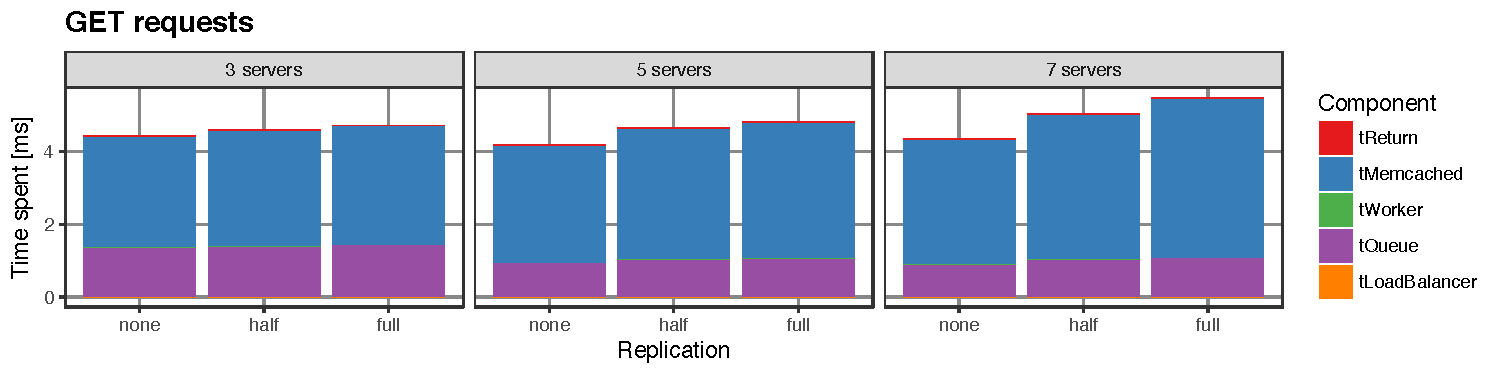
\includegraphics[width=\textwidth]{../results/replication/graphs/time_breakdown_vs_replication_get_abs.pdf}
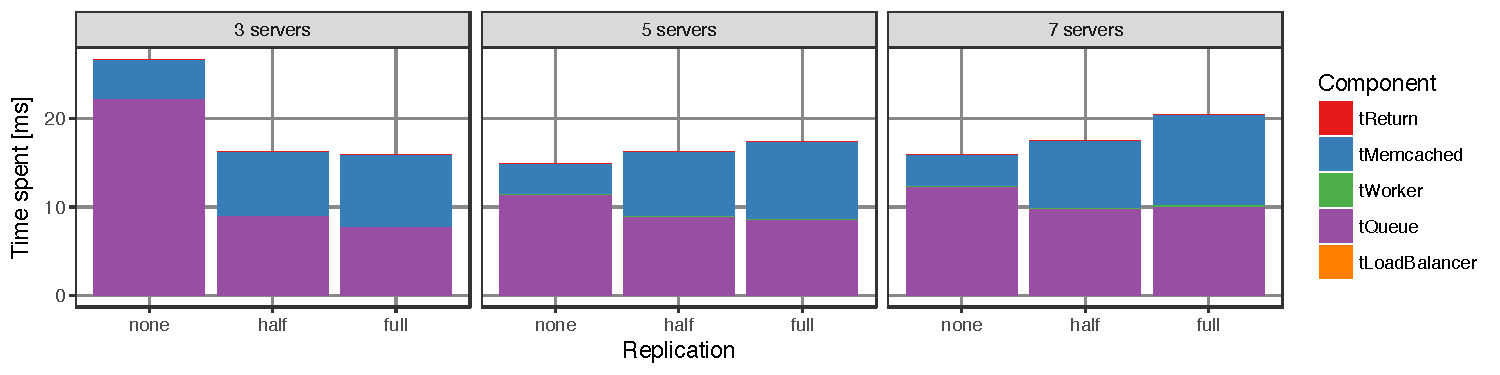
\includegraphics[width=\textwidth]{../results/replication/graphs/time_breakdown_vs_replication_set_abs.pdf}
\caption{Absolute cost of operations inside SUT as a function of $R$, for different values of $S$. Each column is divided into sections by the \emph{average} time spent in the respective component of SUT.}
\label{fig:exp2:res:breakdown}
\end{figure}

\begin{figure}[h]
\centering
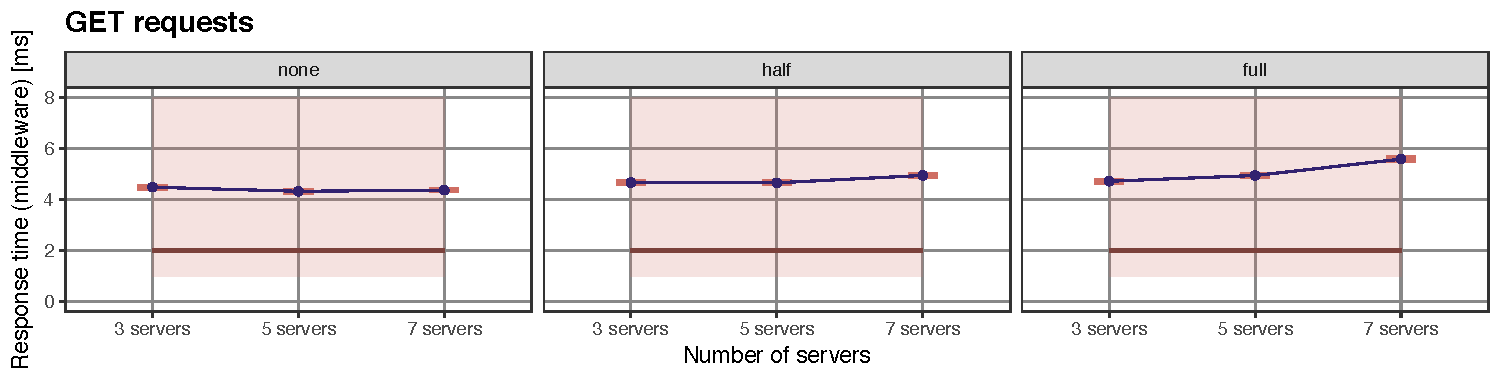
\includegraphics[width=\textwidth]{../results/replication/graphs/response_time_vs_servers_get.pdf}
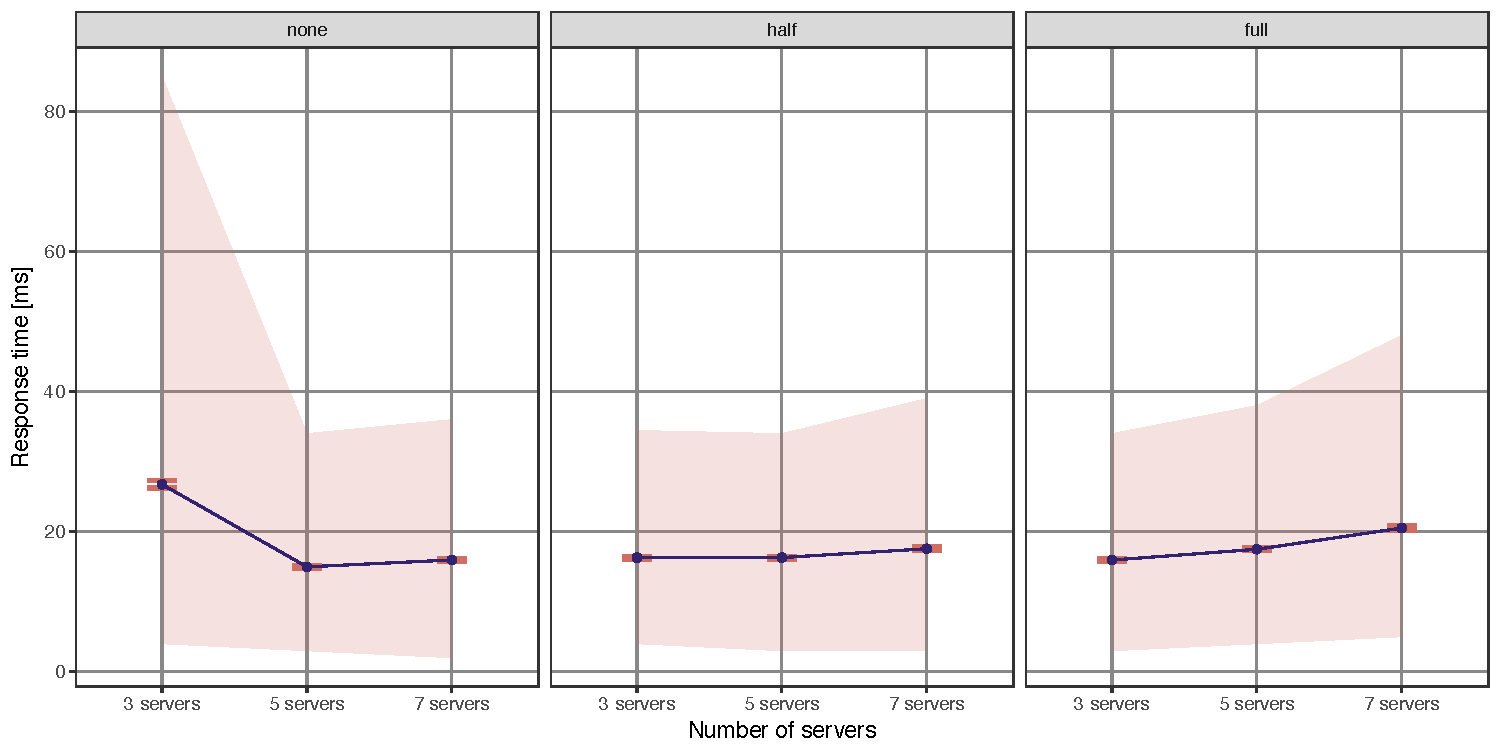
\includegraphics[width=\textwidth]{../results/replication/graphs/response_time_vs_servers_set.pdf}
\caption{Response time (middleware) as a function of $S$, for different values of $R$. The line and points show the mean response time; red errorbars show the 95\% confidence interval in a double-tailed t-test; the light red area shows the 25\% (bottom edge) and 75\% (top edge) quantiles of response times; the red line shows the median.}
\label{fig:exp2:res:servers}
\end{figure}

\subsubsection{Throughput}

From Figure~\ref{fig:exp2:res:throughput} we can see that throughput does indeed decrease with $R$ -- which is in line with the hypothesis --, and higher $S$ amplifies this effect. At $S=3$ throughput is almost constant; this is because the value of $R \in \{1,2,3\}$ does not change enough to make a significant difference, similarly to the previous section. Maximum throughput is achieved at $S=5, R=1$ which is likely because in Section~\ref{sec:exp1} we picked the values of $C$ and $T$ that maximised throughput under exactly those parameters.

\begin{figure}[h]
\centering
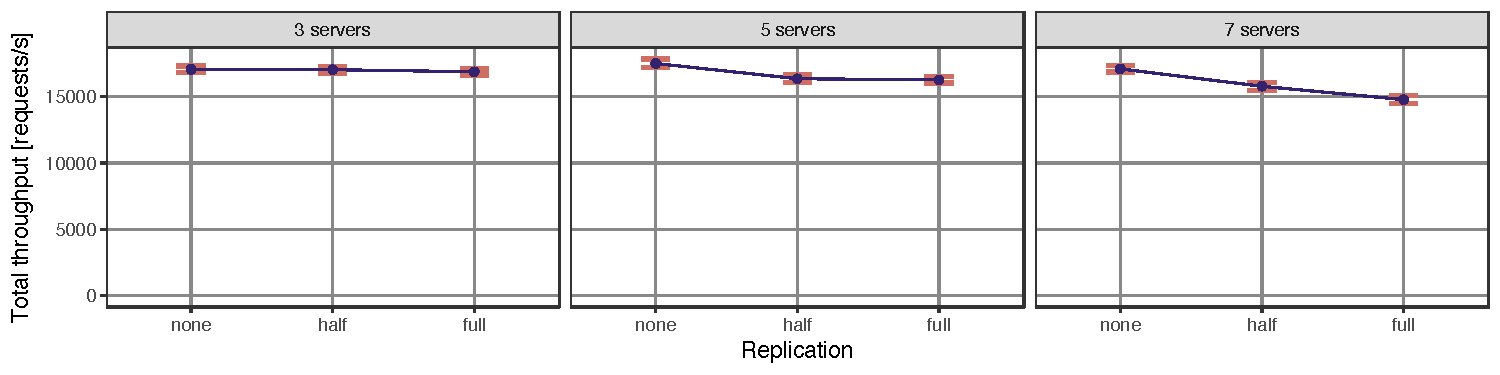
\includegraphics[width=\textwidth]{../results/replication/graphs/tp_vs_replication_all.pdf}
\caption{Throughput of SUT as a function of $R$, for different values of $S$. The line and points show the mean throughput; red errorbars show the 95\% confidence interval over 10-second samples in a double-tailed t-test.}
\label{fig:exp2:res:throughput}
\end{figure}

\subsubsection{Relative cost of operations}
As hypothesized, increasing $R$ also increases $tMemcached$ for \set{} requests. Unexpected though was the decrease in $tQueue$ for \set{} requests as $R$ increased, and the increase in $tMemcached$ for \get{}s. Both are explained in previous sections of this chapter.

\subsubsection{Scalability}
As Figure~\ref{fig:exp2:res:servers} shows, there is no speed-up for \get{} requests when we add servers, and there is even a slight increase the mean response time. Increasing $S$ does decrease mean response time to \set{} requests, but only at $R=1$ and sublinearly -- as hypothesized. At $R>1$ there is no speed-up. In summary, SUT performs significantly worse than the ideal system described in Section~\ref{sec:exp2:hyp:scalability}, and worse than expected.

 \clearpage
% --------------------------------------------------------------------------------
% --------------------------------------------------------------------------------
\section{Effect of Writes}
% --------------------------------------------------------------------------------
% --------------------------------------------------------------------------------
\label{sec:exp3}

\subsection{Experimental question}

In this section, I will run experiments to find out how the response time and throughput of the SUT depend on the proportion of write requests, $W$. I will investigate this relationship for different values of $S$ and $R \in {1, S}$. Finally, I will find out the main reason for the reduced performance.

To this end, I will measure throughput (in 10-second time windows) and response time (for every 10th request) as a function of $W$, $S$ and $R$, and measure how long requests spend in each part of the SUT (based on the timestamps defined in Milestone 1). For each parameter combination, I will run experiments until the 95\% confidence interval (calculated using a two-sided t-test) lies within 5\% of the mean throughput, but not less than 3 repetitions.

\subsection{Hypothesis}

I predict the following.

\subsubsection{\get{} requests}
Increasing $W$ will have no impact on the performance of \get{}s. This is because (assuming SUT is not completely saturated) read threads will have a similar amount of requests to process ($1-W \approx 1$). There may be secondary effects due to e.g. write threads requiring more CPU time, but this should be negligible.

\subsubsection{\set{} requests}
Increasing $W$ will decrease total throughput and increase mean \set{} response time for any combination of $S$ and $R$ because \set{}s take longer to process than \get{}s, and because there are more requests per write thread compared to read threads. Fully replicated setups ($R=S$) will suffer a larger performance decrease than setups with no replication ($R=1$) because in the case of full replication, WriteWorkers do more work for each \set{} request (i.e. the response time of each write request will be higher).

\subsubsection{Relative impact}
The setups with $S=3$ servers will suffer the largest relative performance decrease (compared to $S > 3$) because there are fewer WriteWorkers dealing with the same load of \set{} requests, which in turn increases the queue wait time $tQueue$.

\subsection{Experiments}
\begin{center}
\small{
\smallskip
\begin{tabular}{|c|c|}
\hline Number of servers & $\in \{3, 5, 7\}$ \\ 
\hline Number of client machines & 3 \\ 
\hline Virtual clients & 180 \\ 
\hline Workload & Key 16B, Value 128B, Writes $\in \{1\%, 4\%, 7\%, 10\%\}$ \\
\hline Middleware: replication factor & $\in \{1, S\}$ \\ 
\hline Middleware: read threads & 32 \\ 
\hline Runtime x repetitions & 8min x 3 \\ 
\hline Log files & writes-S*-R*-W*-r* \\
\hline 
\end{tabular} }
\end{center}

\subsection{Results}
Reporting experiment results. Comparison of hypothesis and experiment results.

\subsubsection{Impact on \get{} requests}

Figure~\ref{fig:exp3:res:responsetime} shows the effect of $W$ on \get{} requests. While the mean response time does vary slightly (up to 1ms), the 25\% and 75\% quantiles are relatively stable with one exception. This is roughly as expected (response time does increase slightly with $W$, but this can be attributed to increased network latency because $tQueue$ is stable across parameter combinations).

In the exceptional case, $(S=3,R=1)$, $tQueue$ decreases as $W$ increases. Given that $(S=3,R=3)$ has an otherwise similar behaviour without the decrease in $tQueue$ we can conclude that the decrease is caused by read threads reaching a knee in their performance function: removing just a small proportion of the load gives a large gain in performance.

\subsubsection{Impact on \set{} requests}

Figure~\ref{fig:exp3:res:responsetime} shows the effect of $W$ on \set{} requests, and Figure~\ref{fig:exp3:res:breakdown:set:abs} shows the relative cost of operations inside SUT. It is clear that increasing $W$ also increases response time -- this is in line with the hypothesis. However, the prediction that fully replicated would suffer the most didn't hold: in fact, while response time seems to depend linearly on $W$ in the fully replicated case, the dependence looks exponential in the case of $R=1$. The reasoning for why $R=1$ performs unexpectedly badly (especially for $S=3$) can be found in Section~\ref{sec:exp2:res:set}.

\subsubsection{Throughput}
As Figure~\ref{fig:exp3:res:throughput} shows, throughput does indeed decrease with $W$ for all combinations of $S$ and $R$, confirming the hypothesis. I also predicted that throughput would suffer more for fully replicated setups; this is indeed the case although the difference is not large (the slope of the line in Figure~\ref{fig:exp3:res:throughput} is steeper in plots of the top row compared to the bottom row).

\subsubsection{Relative impact}
I predicted that the largest relative performance decrease would be for a lower number of servers, i.e. $S=3$ would be hit worst by increasing $W$; Figure~\ref{fig:exp3:res:relative:set} confirms this strongly for $R=1$ and mildly for $R=S$.

\subsubsection{Reasons for reduced performance}
Figure~\ref{fig:exp3:res:breakdown:set:abs} shows the relative cost of operations inside SUT

\todo{}

\begin{figure}[p]
\centering
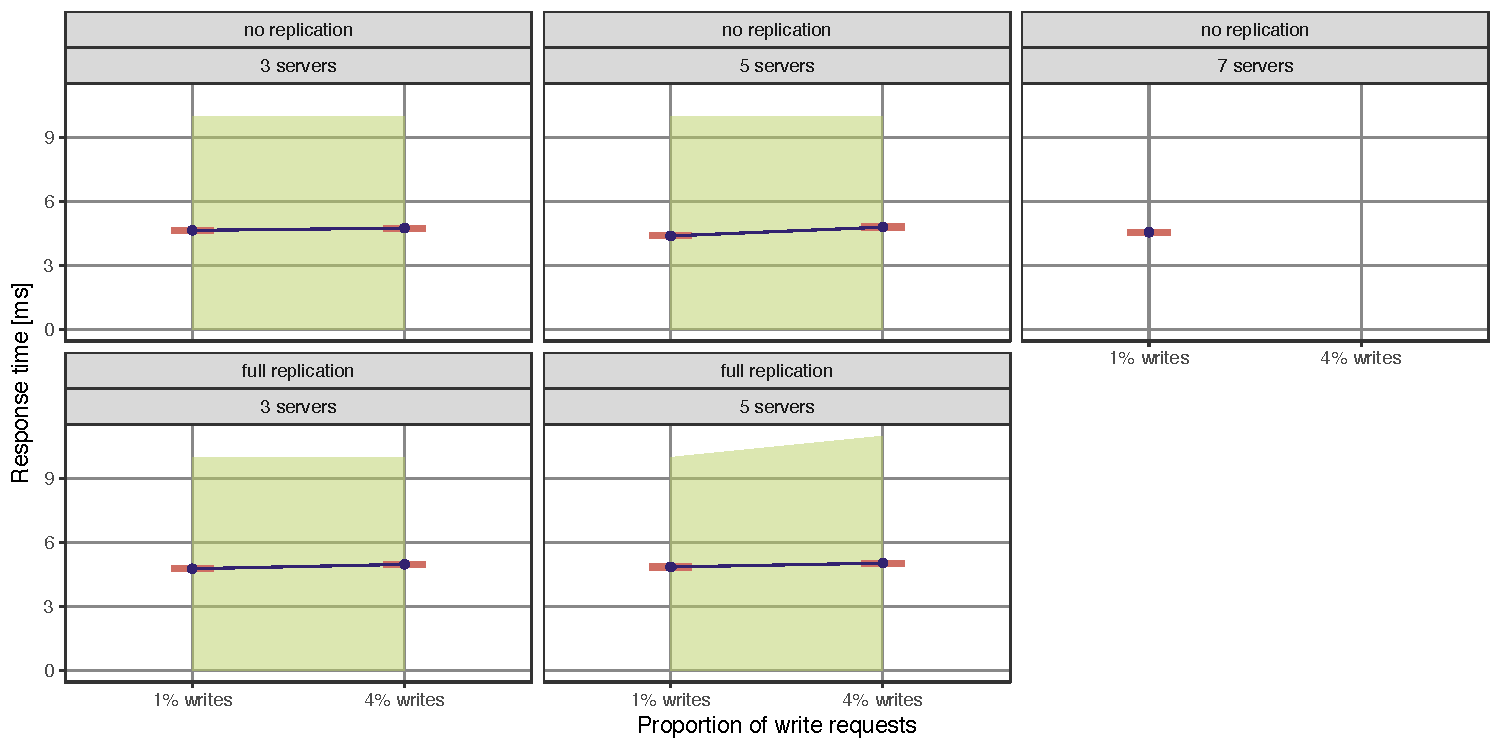
\includegraphics[width=\textwidth]{../results/writes/graphs/response_time_vs_writes_get.pdf}
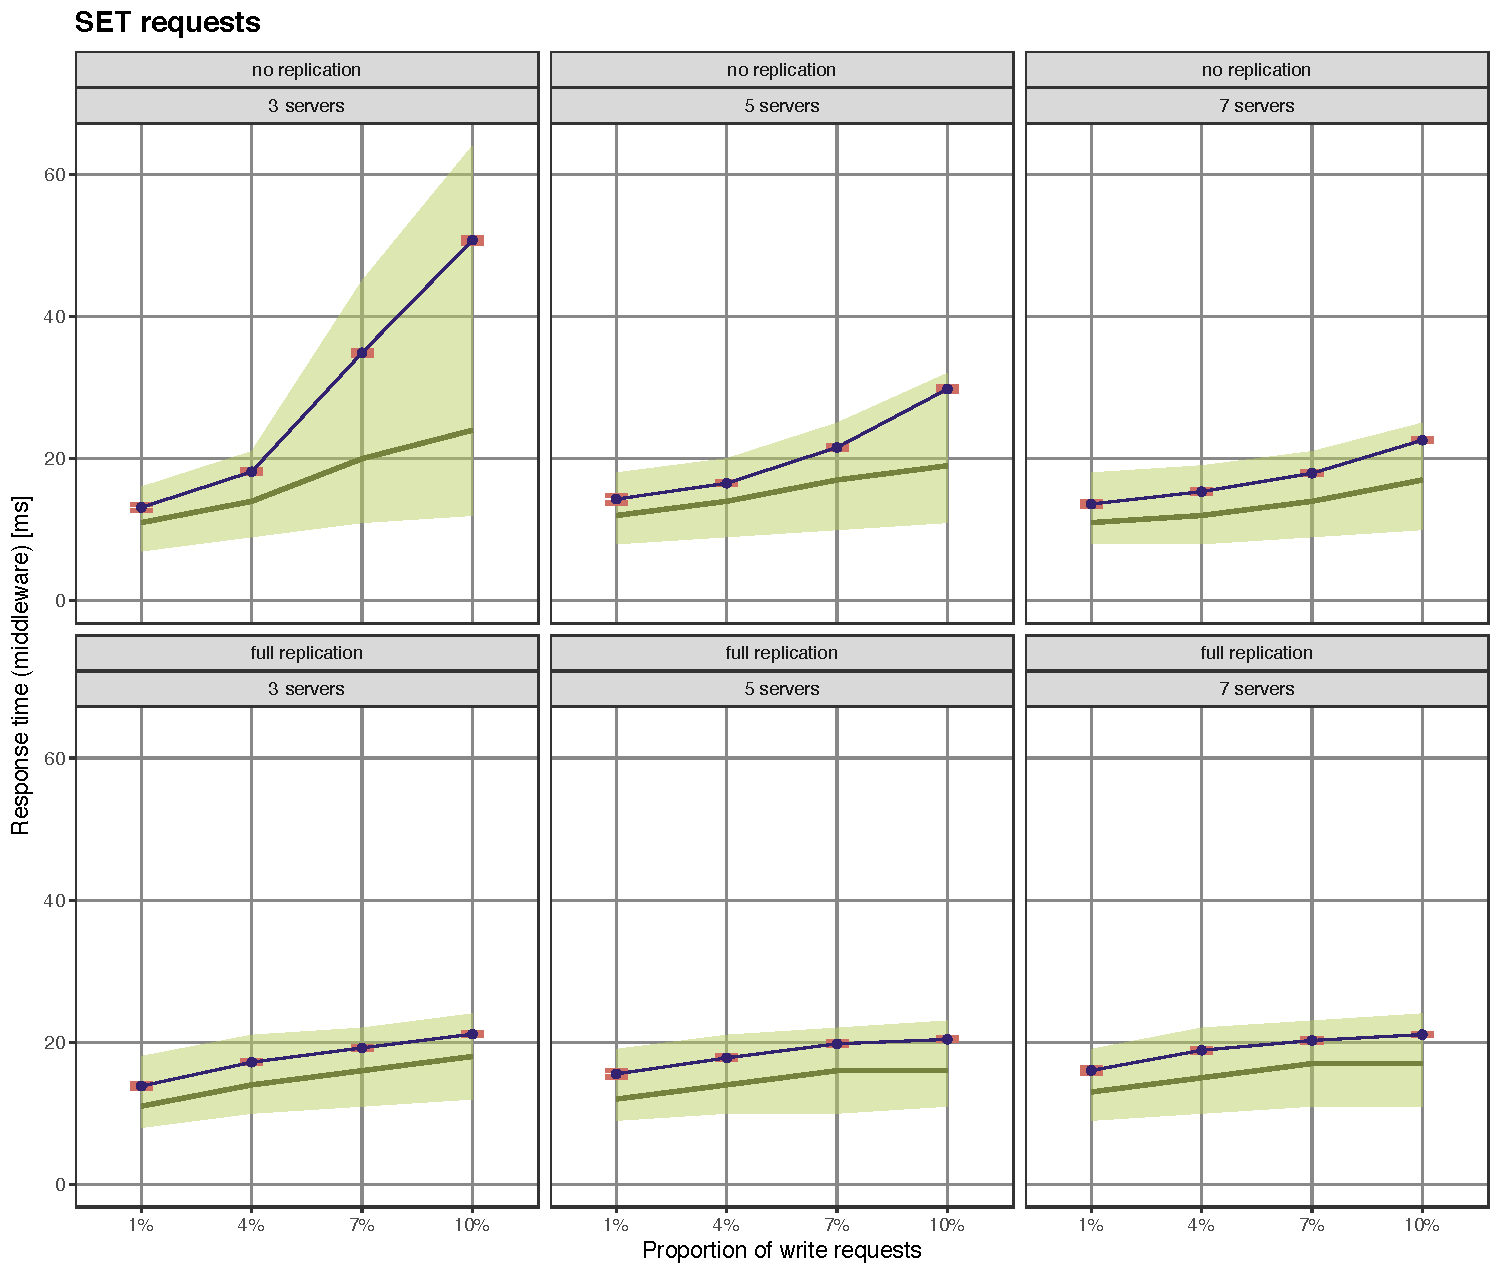
\includegraphics[width=\textwidth]{../results/writes/graphs/response_time_vs_writes_set.pdf}
\caption{Response time (middleware) as a function of $W$, for different values of $S$ and $R$. The blue line and points show the mean response time; red errorbars show the 95\% confidence interval in a double-tailed t-test; the green area shows the 25\% (bottom edge) and 75\% (top edge) quantiles of response times; the green line shows the median.}
\label{fig:exp3:res:responsetime}
\end{figure}

\begin{figure}[h]
\centering
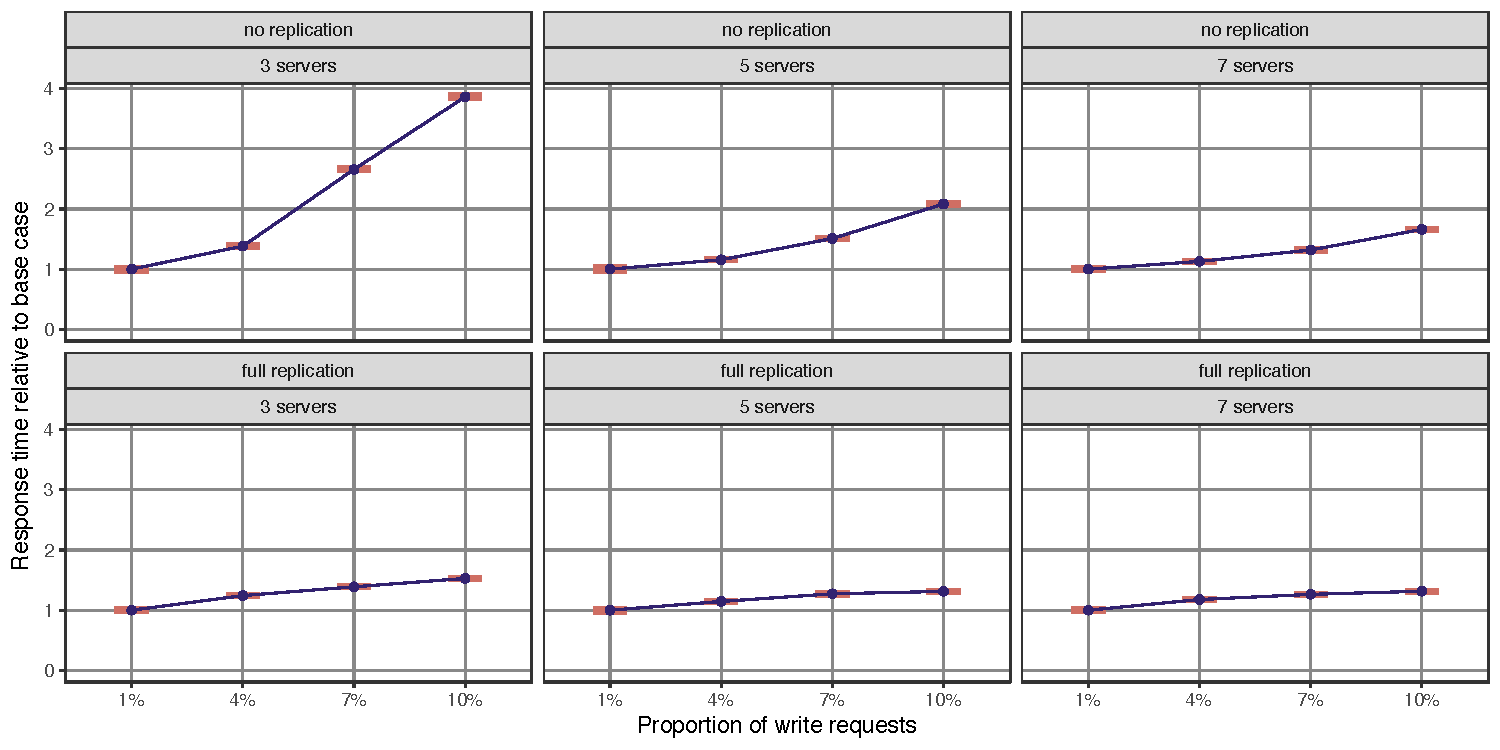
\includegraphics[width=\textwidth]{../results/writes/graphs/relative_performance_set.pdf}
\caption{Relative performance of \set{} requests for different values of $S$ and $R$: the response time (middleware) of each setup relative to (divided by) the response time in the base case. The base case is taken to be $W=1\%$ for each combination of $R$ and $S$.
The line and points show the mean response time; red errorbars show the 95\% confidence interval in a double-tailed t-test.}
\label{fig:exp3:res:relative:set}
\end{figure}

\begin{figure}[h]
\centering
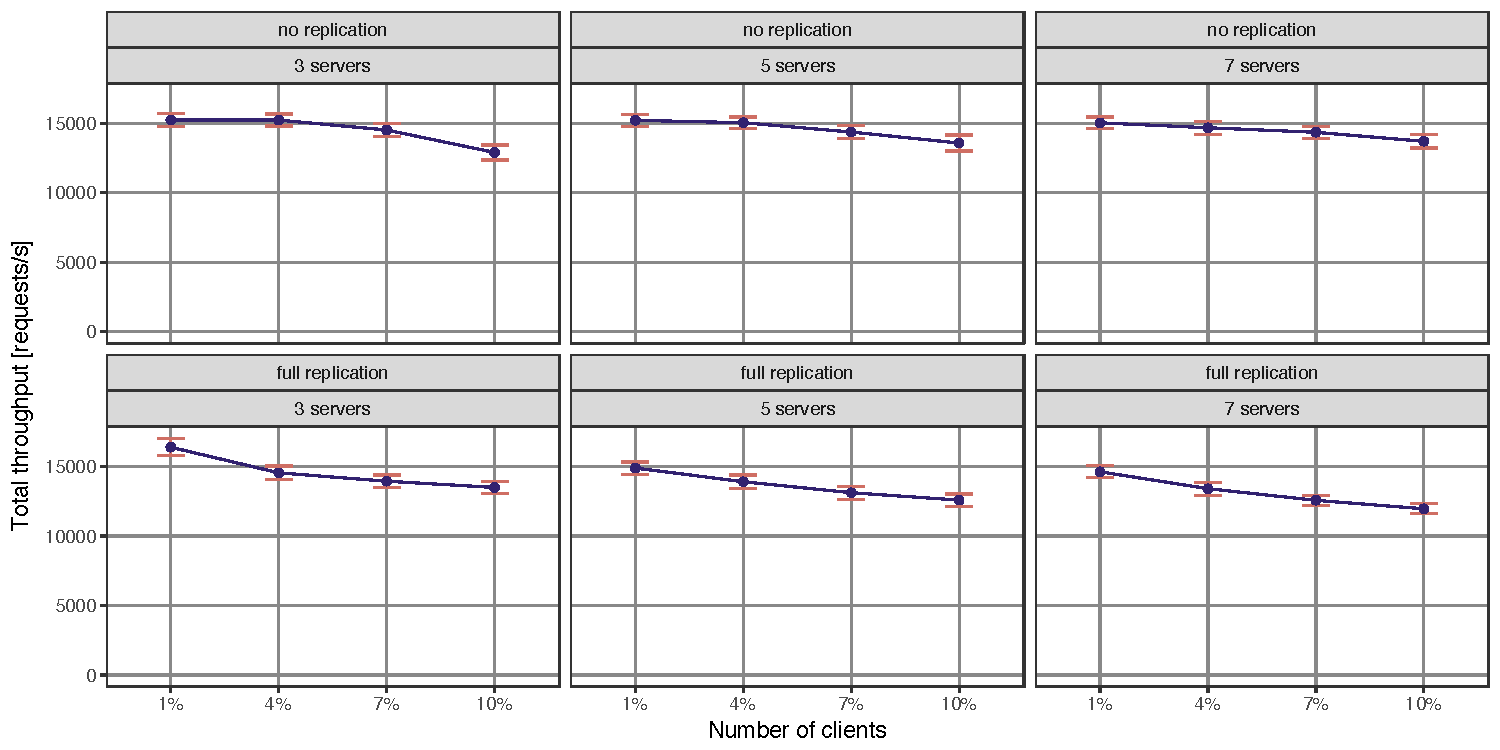
\includegraphics[width=\textwidth]{../results/writes/graphs/throughput_vs_writes.pdf}
\caption{Throughput of SUT as a function of $W$, for different values of $S$ and $R$. The line and points show the mean response time; red errorbars show the 95\% confidence interval over 10-second samples in a double-tailed t-test.}
\label{fig:exp3:res:throughput}
\end{figure}

\begin{figure}[h]
\centering
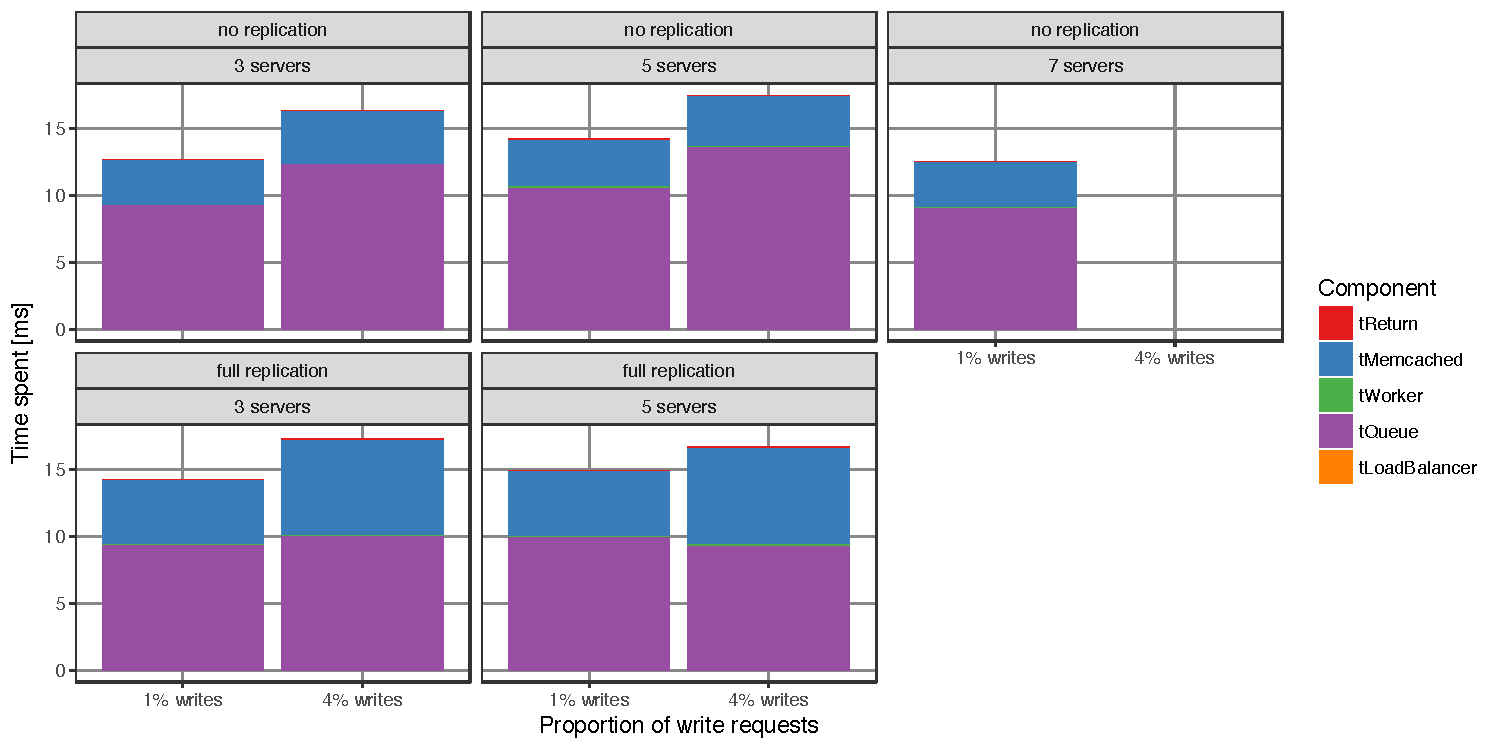
\includegraphics[width=\textwidth]{../results/writes/graphs/time_breakdown_vs_writes_set_abs.pdf}
\caption{Absolute cost of \set{} requests inside SUT, for different values of $S$ and $R$. Each column is divided into sections by the \emph{average} time spent in the respective component of SUT.}
\label{fig:exp3:res:breakdown:set:abs}
\end{figure}

\clearpage

\section*{Appendix A: Comparison of middleware and memaslap data}
\label{sec:appa}
\addcontentsline{toc}{section}{Appendix A: Comparison of middleware and memaslap data}

The response time statistics that memaslap outputs are useful but limited. Since using middleware data allows studying the response time distribution in more detail, we would like to use response times measured by the middleware. To do this, however, we need to show that these two are interchangeable up to a constant delay caused by the network latency on the roundtrip between memaslap and the middleware.

Figures~\ref{fig:appa:comparison:exp2} and \ref{fig:appa:comparison:exp3} show the mean response times as measured by memaslap and the middleware. It is clear that for all parameter combinations, the difference is indeed constant at about 5ms. Thus, we can rely on response times logged by the middleware.

\begin{figure}[h]
\centering
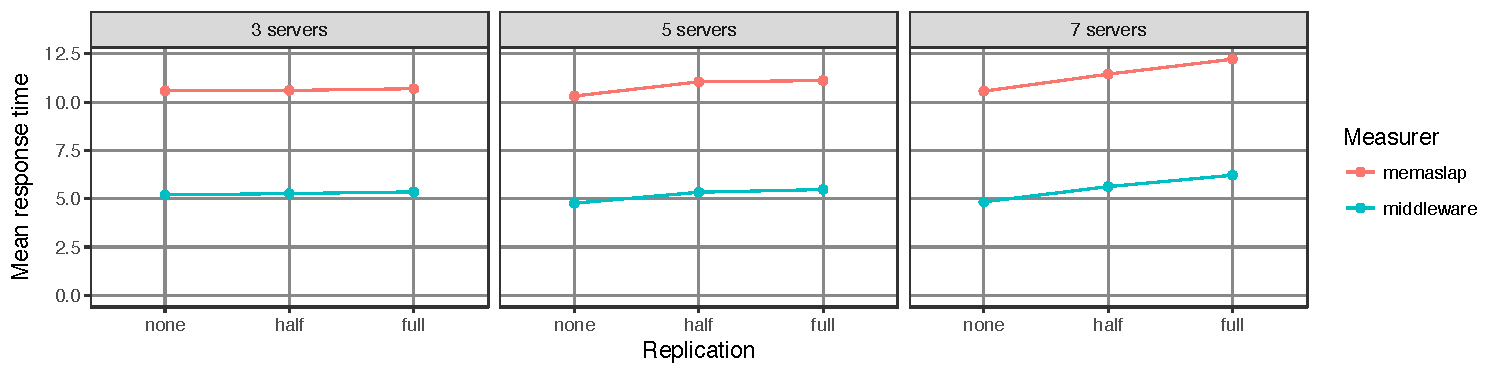
\includegraphics[width=\textwidth]{../results/replication/graphs/compare_mw_ms.pdf}
\caption{Mean response time as measured by memaslap and middleware in all experiments of Section~\ref{sec:exp2}.}
\label{fig:appa:comparison:exp2}
\end{figure}

\begin{figure}[h]
\centering
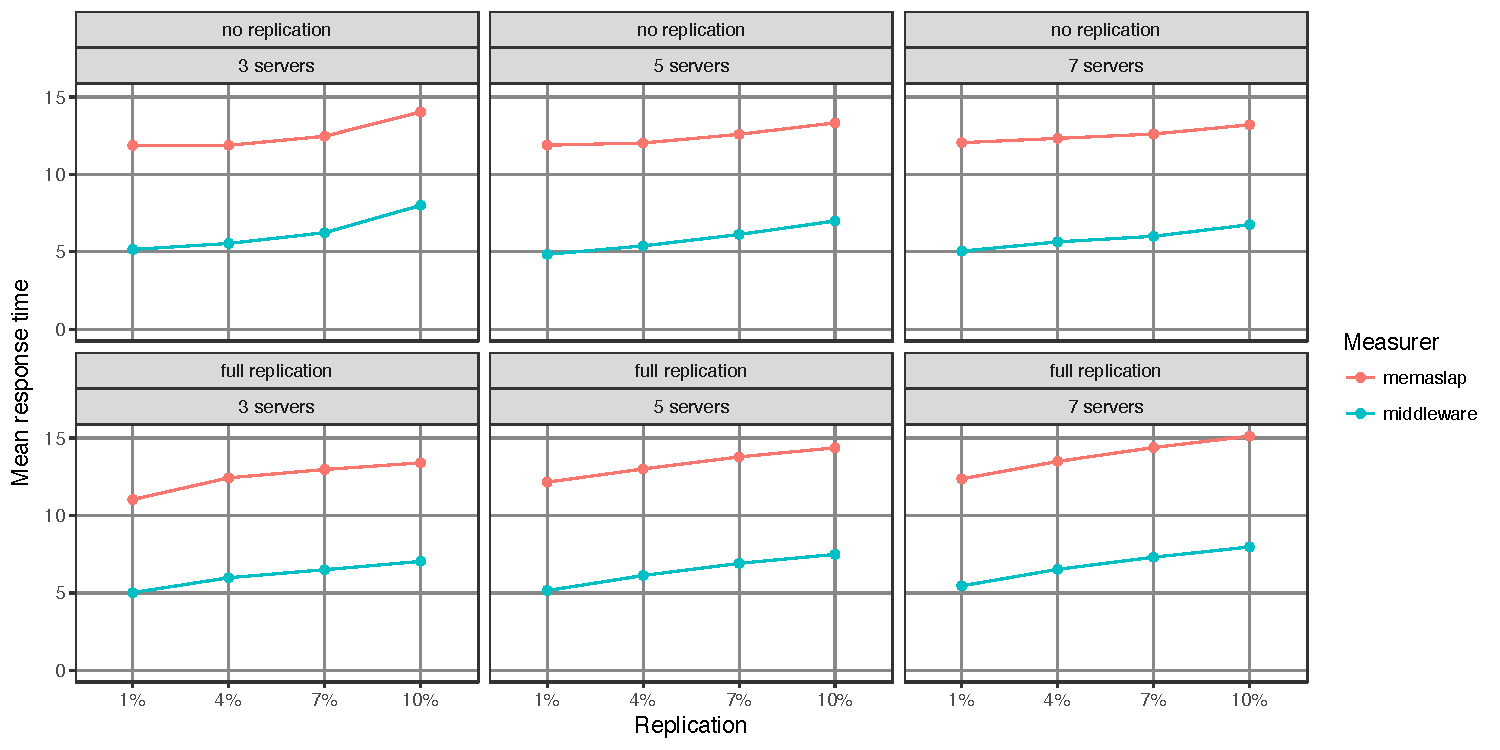
\includegraphics[width=\textwidth]{../results/writes/graphs/compare_mw_ms.pdf}
\caption{Mean response time as measured by memaslap and middleware in all experiments of Section~\ref{sec:exp3}.}
\label{fig:appa:comparison:exp3}
\end{figure}



\clearpage

\section*{Log file listing}
\addcontentsline{toc}{section}{Log file listing}

Each experiment's logs are compressed into one or more \verb+compressed.zip+ files and should be extracted to the directory where the \verb+.zip+ file is located. Each location mentioned in the table below is a directory that contains the middleware log (\verb+main.log+), the request log (\verb+request.log+) and memaslap outputs (\verb+memaslap*.out+). \\

\begin{tabular}{|c|l|}
\hline \textbf{Short name}& \textbf{Location} \\ 
\hline throughput-C*-T*-r* & \href{https://gitlab.inf.ethz.ch/pungast/asl-fall16-project/blob/master/results/throughput}{gitlab.inf.ethz.ch/.../results/throughput/clients*\_threads*\_rep*} \\ 
\hline replication-S*-R*-r* & \href{https://gitlab.inf.ethz.ch/pungast/asl-fall16-project/blob/master/results/replication}{gitlab.inf.ethz.ch/.../results/replication/S*\_R*\_rep*} \\ 
\hline writes-S*-R*-W*-r* & \href{https://gitlab.inf.ethz.ch/pungast/asl-fall16-project/blob/master/results/writes}{gitlab.inf.ethz.ch/.../results/writes/S*\_R*\_writes*\_rep*} \\ 
\hline 
\end{tabular} 
 
\end{document}